% Conclusion

\chapter{Conclusions and Perspectives} % Write in your own chapter title
\label{Conclusion}
%\addtotoc{Conclusion and perspectives}
\lhead{\emph{Conclusions and Perspectives}} % Write in your own chapter title to set the page header

\section{Conclusions}
In this thesis, we considered state detection and load disaggregation, which can be implemented by three main approaches:
\begin{itemize}
\item Intrusive load monitoring: the sensors (including the power meters and the environment monitoring sensors) are attached to each individual device. This approach obviously shows a high accuracy, but requires a high cost as well as too much technical intervention on the power supply to deploy the sensors.
\item Non-intrusive load monitoring: this approach is promising to study because it requires only one power meter installed at the main power entry to measure the power consumption of all devices. The aggregate power signal is then analyzed to extract the specific features to identify the operation of the corresponding devices. The selection of features depends on the sampling frequency of the meters, divided into two groups:
\begin{itemize}
\item High frequency: the features relate to the transient signal waveform, e.g. \textit{v-shape}, or the Fourier transform of the stable signal, e.g. harmonics.
\item Low frequency: basically corresponding to the power signal of the steady state such as average power, step-changes of length of each steady duration.
\end{itemize}
Apparently, high-frequency based methods can benefit from more characteristics of the devices and show a higher quality of detection than the low frequency approaches. However, the price of the hardware also increases along with the frequency and the identification is more complex. For example, it is necessary to transform the signal before applying the algorithms.
\item Hybrid load monitoring: to improve the performance of the NILM algorithms, some additional information such as acoustic noise, light intensity, occupancy can be used to detect the operation of some specific devices. Obviously, this approach leads to a high cost than NILM, but it is still less intrusive.
\end{itemize}

In our work, in Chapter~\ref{l1norm}, we firstly try to solve the $l1$-norm minimization problem in NILM by a brute force algorithm. This method sequentially tests all combinations of states to find one giving the minimum absolute error between the aggregate power and total power demand of the identified devices. Obviously, this algorithm cannot show a good performance if there are devices with the same or near power demand. Therefore, instead of selecting the combination with the least error, we proposed to keep all combinations giving an error around the least value and compare with the previous state of the devices to determine the final solution. The comparison can be based on the distance from the previous state and the current state or the state transition probability between them. The simulation results with the Athemium data, retrieved by monitoring some devices in our coffee room, show that the performance can be significantly improved by these two versions of the brute force algorithm.

The main contribution of this thesis is presented in Chapter~\ref{SmartSense} with a hybrid load monitoring system called SmartSense, in which a WSN is deployed to monitor some specific devices and provide their operating probability. There are two approaches 
proposed to combine the probability feature with the NILM algorithms, including:
\begin{itemize}
\item Knapsack approach: formulated by combining the probability of the devices with the minimization problem in NILM. The Knapsack problem is then solved by a compositional Pareto-algebraic heuristic (CPH) or a dynamic programming (DP) algorithm.
\item Edge detector approach: an edge detector is applied to detect the rising edges and falling edges of an activation on the power signal to create the features. The probability information of each device is then combined with these features by a regularization parameter to form new more effective ones. If the ED algorithm is applied, the features comprise only the rising edge and falling edge, while in the DTW one, all active power values between these edges are retained. 
\end{itemize}

In Chapter~\ref{ResultsSS}, the proposed algorithms are simulated with four dataset including two houses from REDD, one house in UK-DALE and our Athemium data. The results show that the performance can be significantly improved by monitoring a part of devices. Besides, there are several parameters affecting the performance of the algorithms in SmartSense, such as type and number of monitored devices or the reliability of the sensor network. The selection of these parameters needs to make balance between the desired performance and the cost of WSN deployment.
Besides, the computational complexity is also necessary to be considered. Despite performing a higher performance with more than two monitored devices, the CPH and DP algorithms require a larger amount of computations than the ED and DTW ones. 

\begin{figure}[h]
\centering
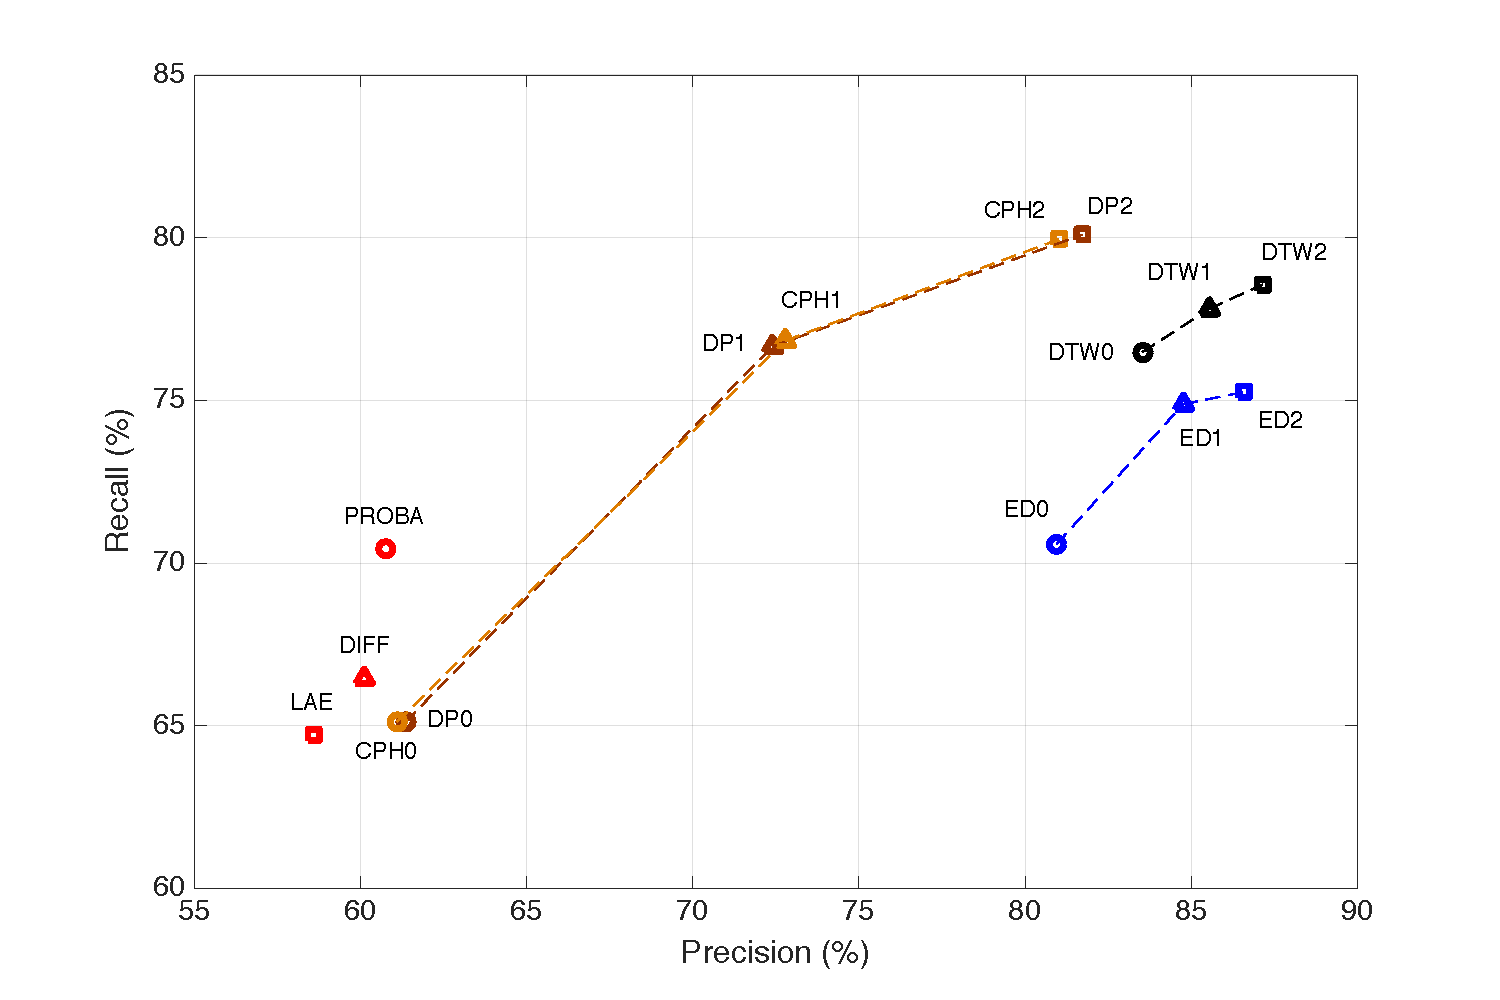
\includegraphics[width=1\textwidth]{./chapters/Conclusion/all_perfcomp.pdf} 
\caption{Performance of all proposed algorithms with REDD dataset \emph{House 1}. The index following the algorithms denotes the number of monitored devices.} 
\label{fig:C1} 
\end{figure}

\par In Figure~\ref{fig:C1}, performance of all proposed algorithms in this thesis with REDD dataset \emph{House 1} is presented. The least absolute error based algorithm (LAE), state difference based algorithm (DIFF) and state transition probability based algorithm (PROBA) are introduced in Chapter~\ref{l1norm}. Meanwhile, the four proposed algorithms in SmartSense with one monitored device (DP1, CPH1, ED1, DTW1) and two monitored devices (DP2, CPH2, ED2, DTW2) are compared with the corresponding algorithms in state of the art (DP0, CPH0, ED0, DTW0). The three $l1$-norm minimization based algorithms introduced in Chapter~\ref{l1norm} (LAE, DIFF, PROBA) show the worst detection. Meanwhile, in the SmartSense system, although CPH and DP show a worse performance when applied in traditional NILM, the algorithms used in the knapsack approach are more significantly improved than the edge detector algorithms (DTW1, DTW2, ED1, ED2) when several devices in home are monitored by the WSN (DP1, DP2, CPH1, CPH2). In addition, they also outperform other algorithms in term of sensibility (recall) with more than one monitored devices.


\section{Perspectives}

Along with the development of smart homes and smart buildings, load monitoring becomes one of the most important issues, in which non-intrusive approach is the more promising because of less technical intervention on the power supply. Sensor-aided NILM or SmartSense, can become an efficient model for NILM researches because it can significantly improve performance of existing NILM algorithms with the deployment of several low-cost, low-power and less complicated sensors to monitor a subset of all devices in home or building. For example, the operation of the fridge compressor can be easily detected by a vibration sensor, while the lighting system can be monitored by a light sensor. These sensors do not require too much technical intervention and the users can easily install the sensors by themselves. As a consequence, the intrusive requirement is still respected, which is quite different from the intrusive load monitoring such as ViridiScope~\cite{Kim09Ubicomp}. In addition, because the detection of sensors is used to estimate the operating probability of corresponding devices and used as an additional information in NILM algorithms, effect of false detection can be reduced. 
\par Using sensors to monitor the operation of electrical devices has been developed for many decades. Moreover, the appearance of the electrical devices with embedded sensors such as smart televisions, smart lamps, etc., allows the SmartSense model to be deployed more conveniently. The opportunities for extending the scope of this thesis correspond to the development of disaggregation algorithms as well as the improvement of probability estimation.
\par The most significant advantage of the SmartSense model is the reuse of existing NILM algorithms. In this thesis, we applied the SmartSense idea to the edge detector algorithms, which is the first approach of NILM proposed by G.~Hart~\cite{Hart92}, and the proposed knapsack approach to solve the $l1$-norm minimization problem in NILM. The SmartSense model shows results with significant improvements thanks to the different proposed algorithms. Of course, other approaches can also be applied in SmartSense such as HMM, ANN, deep learning neural networks, etc. Concretely, in any HMM, emission probability and transition probability are two of the most important parameters to be learned. When applied in SmartSense, the emission probability corresponding to each state can be studied to be replaced by the operating probability estimated by the WSN. Meanwhile, with ANN or deep learning neural network, the operating probability of each device can be considered as an input, along with the aggregate power measurement, to determine the state of devices at the output. The number of hidden layers and the structure of the network are principal issues to be studied in future work. Besides, we also need to study self-training algorithms, which are able to automatically learn the parameters by an adaptive process without training data. Algorithm which can be applied to the devices with variable loads is also an important issue.
\par In the knapsack approach of this thesis, the operating probability of each state strongly depends on the number of states of each device. This becomes a problem if a device has too many operating states. Because of being divided by the number of states, the operating probability of each state becomes very low although the corresponding device is detected as being switched on with high reliability. Therefore, developing an algorithm for probability estimation in order to eliminate the effect of the number of states also needs to be studied in future work. Additionally, we also need to deploy a WSN in certain rooms to verify the operation of SmartSense in real condition instead of simulating with publicly dataset. This will be done during 2017 in the context of the SmartSense platform deployment funded by INRIA and the "Region Bretagne" in the context of the CPER SmartSense funding. 
